\documentclass[hyperref={pdfpagelabels=false},table]{beamer}
%\documentclass{beamer}
\usepackage{../estilo-apresentacao/slides-utfpr}

%\hypersetup{pdfpagemode=FullScreen}   %%% para deixar no modo de tela cheia
\beamertemplatenavigationsymbolsempty   %%% para não mostrar ícones de navegação no canto direito inferior

% Nome da disciplina - informação que somente aparece nas propriedades do arquivo PDF
\subject{Desenvolvimento de Aplicaç\~{o}es Distribu\'{i}das - UTFPR}

\title[Desenv. Apl. Distribu\'{i}das - AD23S - 2018/2]{Desenvolvimento de Aplicaç\~{o}es Distribu\'{i}das}
\subtitle{Desafios para a Construç\~{a}o de Sistemas Distribu\'{i}dos}
\author[Prof. Dr. F\'{a}bio Favarim]{Prof. Dr. F\'{a}bio Favarim \texorpdfstring{\\ \footnotesize{favarim@utfpr.edu.br}}{}}
\institute[UTFPR]{ 
\small{\textbf{Universidade Tecnológica Federal do Paraná}}\\
Câmpus Pato Branco
}

\date{7 de Agosto de 2018}

\begin{document}

\begin{frame}
	\titlepage
\end{frame}

\begin{frame}[wide]
	\frametitle{Objetivos da Aula}
   \begin{block}{}
		\begin{itemize}
		  \item Conhecer os desafios para a construção de sistemas distribuídos e as Transparências desejáveis em sistemas distribuídos;
		  \item Conhecer o que é middleware e sua importância;
		  \item Conhecer as arquiteturas de sistemas distribuídos.
		\end{itemize}
   \end{block}
\end{frame}


%%% Sumário
\begin{frame}
	\frametitle{Sumário}
	\small
	\tableofcontents
	\normalsize
\end{frame}


\section*{Revisão aula passada}

\begin{frame}[wide]
	\frametitle{Introdução aos Sistemas Distribuídos}
	\framesubtitle{Revisão da Primeira Aula}
	\begin{itemize}
		\item \textbf{Algumas aplicações são nativamente distribuídas}
		\begin{itemize}
			\item mensagens instantâneas, sistema acadêmico, navegação web
		\end{itemize}
		\item \textbf{Desempenho}
		\begin{itemize}
			\item Tarefas podem ser distribuídas por diversos computadores
			\item Facilidade para aumentar a capacidade de processamento (número de CPU)
			\item Vantagem financeira: Desempenho \textit{vs} Custo
		\end{itemize}
		\item \textbf{Algumas aplicações são críticas}
		\begin{itemize}
			\item Continuará funcionando mesmo diante de alguma falha
		\end{itemize}
	\end{itemize}
\end{frame}


\begin{frame}[wide]
	\frametitle{Introdução aos Sistemas Distribuídos}
	\framesubtitle{Revisão da Primeira Aula}
	\textbf{Dificuldades em sistemas distribuídos}
		\begin{itemize}
			\item Compartilhamento
			\begin{itemize}
				\item Dados e processamento
			\end{itemize}
			\item Descoberta de serviços
			\begin{itemize}
				\item Como localizar os serviços e depois como invocá-los?
			\end{itemize}
			\item Complexidade para codificação
			\begin{itemize}
				\item Dimensão do sistema e funcionamento não determinístico
			\end{itemize}
		\end{itemize}
\end{frame}

\begin{frame}[wide]{Introdução aos Sistemas Distribuídos}
	\framesubtitle{Revisão da Primeira Aula}
	\textbf{Falhas nos sistemas}
		\begin{itemize}
			\item \textbf{Sistema não distribuído}
			\begin{itemize}
				\item Falha tudo ou nada
				\item O usuário fica ciente da falha
				\item Estratégia de recuperação: fechar e abrir novamente
			\end{itemize}
			\item \textbf{Sistema distribuído}
			\begin{itemize}
				\item Falha pode ser parcial
				\item Falha pode não ser percebida pelo usuário
				\item Diferentes estratégias para lidar com falhas
			\end{itemize}
	\end{itemize}
\end{frame}




% ------------ Inicio da Apresentação ---------------%
\section{Desafios para a Construção de Sistemas Distribuídos}

\begin{frame}
  \frametitle{Desafios para a Construção de Sistemas Distribuídos}
      Os SD são facilmente encontrados em qualquer lugar nos dias de hoje, mas projetos ambiciosos podem pedir requisitos que trazem muitos desafios para o seu desenvolvimento:
      \begin{itemize}
	  \item Heterogeneidade
	  \item Abertura
	  \item Concorrência
	  \item Segurança
	  \item Escalabilidade
	  \item Tratamento de falhas
	  \item Transparência
      \end{itemize}
\end{frame}


\subsection{Heterogeneidade}

\begin{frame}[wide]
  \frametitle{Desafios para a Construção de Sistemas Distribuídos}
  \framesubtitle{Heterogeneidade}
      \begin{block}{}
	Permitir ao sistema funcionar mesmo levando em conta a diversidade de hardware e software.
    \end{block}
  
  \begin{itemize}
      \item Um sistema distribuído deve considerar:
      \begin{itemize}
	  \item diferentes tipos de rede
	  \item diferentes tipos de hardware (diferentes representações de dados, diferente código máquina)
	  \item diferentes sistemas operacionais (diferentes interfaces para os protocolos de comunicação)
	  \item diferentes linguagens de programação (diferentes representações de estruturas de dados como arrays ou registos,...)
      \end{itemize}
      \alert{\item \textbf{Como tratar do problema?}}
  \end{itemize}
\end{frame}


\subsection{Abertura}

\begin{frame}
    \frametitle{Desafios para a Construção de Sistemas Distribuídos}
    \framesubtitle{Ser Aberto / Abertura (Openness)}
    \vspace{-1mm}
    \begin{block}{}
	Permitir ao sistema ser estendido ou implementado de diferentes maneiras
    \end{block}
    \begin{itemize}
	\vspace{-1mm}
	\item \textbf{Exemplos:}
	\begin{itemize}
	    \item \textbf{Computador pessoal} -- É possível adicionar periféricos de diferentes fabricantes
	    \item \textbf{Rede TCP/IP} -- computadores com diferentes arquiteturas e sistemas operacionais conseguem interagir sem problema
	\end{itemize}
	\item Para isso é importante que:
	    \begin{itemize}
		\item publicação de \textbf{interfaces} \vspace{-1mm}
		\item documentação e especificação 	\vspace{-1mm}
		\item código aberto			\vspace{-1mm}
		\item protocolos e formatos padronizados usados na Internet (\textit{Request For Comments} -- RFCs) podem ser obtidas em \url{www.ietf.org}
	    \end{itemize}
	\end{itemize}

	\vspace{-2mm}
	\begin{block}{Sistema Distribuído Aberto}
	\begin{itemize}
		\item Faz uso de mecanismos de comunicação padronizados e torna público  interfaces para acesso aos recursos compartilhados \vspace{-1mm}
		\item Pode ser construído com hardware e software heterogêneos, possivelmente de diferentes fabricantes
	\end{itemize}
	\end{block}
\end{frame}

\subsection{Concorrência}

\begin{frame}
    \frametitle{Desafios para a Construção de Sistemas Distribuídos}
    \framesubtitle{Concorrência}

    \begin{block}{}
	   Permitir que recursos compartilhados possam ser acessados por diversos usuários/processos \alert{simultaneamente}.
    \end{block}	
	
    \begin{itemize}
	\item Questões:
	\begin{itemize}
	    \item Necessário coordenar o acesso aos recursos compartilhados: hw, sw, dados

	    \item \textbf{Problema:} ocorrência de conflitos $\Longrightarrow$ podem gerar inconsistências em ambientes concorrentes. 
	    \begin{itemize}
		\item Dois usuários estão no mesmo momento acessando a mesma tabela no Banco de Dados
		\item O sistema deverá garantir o acesso concorrente ao mesmo tempo que garante a consistência dos dados (geralmente protegidos por \textit{locks}) 
	    \end{itemize}
	\end{itemize}
    \end{itemize}
\end{frame}

\subsection{Escalabilidade}
\begin{frame}
    \frametitle{Desafios para a Construção de Sistemas Distribuídos}
    \framesubtitle{Escalabilidade}
    \begin{block}{}
	   Capacidade do sistema permanecer efetivo mesmo quando há um aumento no número de recursos e usuários.
    \end{block}	
    \begin{itemize}
	\item Um sistema e seu software não deveria mudar severamente seu comportamento quando sua escala (seu ``\textbf{tamanho}'') cresce
	\item Deve-se tomar cuidado com serviços, dados e algoritmos centralizados:
    \end{itemize}

    \begin{center}
      \rowcolors[]{1}{blue!20}{blue!10}
      \begin{tabular}{cp{7cm}} \hline
		Conceito & Exemplo \\ \hline \hline
		Serviços Centralizados & Um único servidor para todos os usuários \\
		Dados Centralizados & Uma única lista telefônica online  \\
		Algoritmos Centralizados & Fazer roteamento com base em informações completas\\
		\hline
      \end{tabular}
    \end{center}
    
    \begin{itemize}
	\item Podem se tornar gargalos, pontos únicos de falhas e saturar a rede onde residem.
    \end{itemize}
\end{frame}

\subsection{Tratamento de Falhas}
\begin{frame}
    \frametitle{Desafios para a Construção de Sistemas Distribuídos}
    \framesubtitle{Tratamento de Falhas}
	\begin{block}{Prevenir}
	     Para que falhas não afetem outros componentes do sistema (física, software e humanas)
	\end{block}
	\begin{block}{Tolerar}
	    Na Web, por exemplo, os browsers são projetados para tolerar falhas. Quando um servidor não pode ser conectado, o browser não fica eternamente tentando estabelecer uma conexão, ao invés disso, ele encerra a tentativa de conexão e em seguida avisa o usuário sobre a desistência;
	\end{block}
	\begin{block}{Recuperação}
	     Dependendo do software, um projeto adequado permite que um sistema possa recuperar um estado consistente de dados até o momento antes da falha. Ex: transações usado em BDs.
	\end{block}
\end{frame}

\begin{frame}
    \frametitle{Desafios para a Construção de Sistemas Distribuídos}
    \framesubtitle{Tratamento de Falhas}
	\begin{block}{Redundância}
	    Os sistemas podem também oferecer componentes redundantes para evitar falhas. Ex: BDs com replicação de dados, Servidores de DNS e Roteadores.
	\end{block}
\end{frame}

\subsection{Segurança}
\begin{frame}
    \frametitle{Desafios para a Construção de Sistemas Distribuídos}
    \framesubtitle{Segurança}	
	\begin{itemize}
	   \item Questão problemática em sistemas distribuídos devido à facilidade de compartilhamento de recursos.
	   \item Segurança costuma ser subdividida em 3 partes:
	\end{itemize}
	\begin{block}{Confidencialidade}
          Proteção contra acesso não autorizado;
	\end{block}
	\begin{block}{Integridade}
         Proteção contra alteração não autorizada
	\end{block}
	\begin{block}{Disponibilidade}
         Proteção contra interferência no acesso ao recurso
	\end{block}
\end{frame}

\begin{frame}
    \frametitle{Desafios para a Construção de Sistemas Distribuídos}
    \framesubtitle{Segurança}	
	\begin{block}{Comunicação normal}
         \textbf{Através de canais de comunicação \alert{não seguros.}}
	\end{block}
	\begin{figure}
	  \centering
	  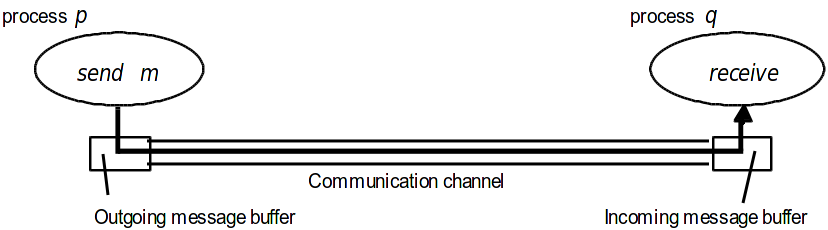
\includegraphics[scale=.4]{figs/seguranca1}
	\end{figure}
\end{frame}

\begin{frame}
    \frametitle{Desafios para a Construção de Sistemas Distribuídos}
    \framesubtitle{Segurança}	
	\begin{block}{}
         \textbf{Interceptação/Alteração da mensagem}
	\end{block}
	\begin{figure}
	  \centering
	  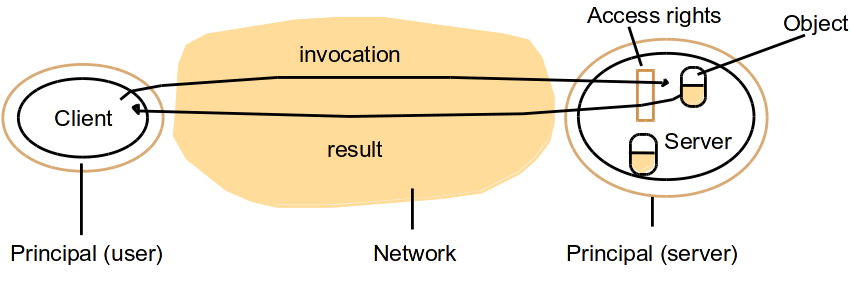
\includegraphics[scale=.3]{figs/seguranca2} \\

	  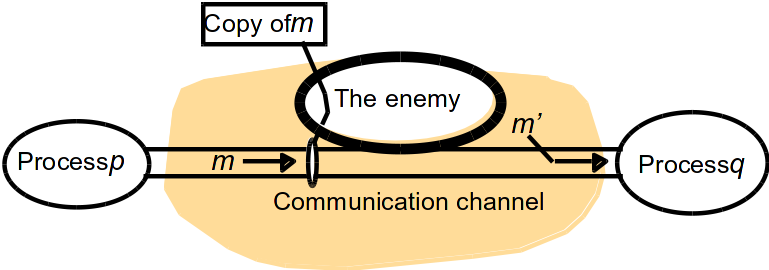
\includegraphics[scale=.3]{figs/seguranca3}
	\end{figure}
\end{frame}




\begin{frame}
    \frametitle{Desafios para a Construção de Sistemas Distribuídos}
    \framesubtitle{Segurança}	

	\begin{block}{Comunicação ``Segura''}
         \textbf{Através de canais de comunicação \alert{seguros.}}
	\end{block}
	\frametitle{Desafios Sistemas Distribuídos - Segurança}
	\begin{figure}
	  \centering
	  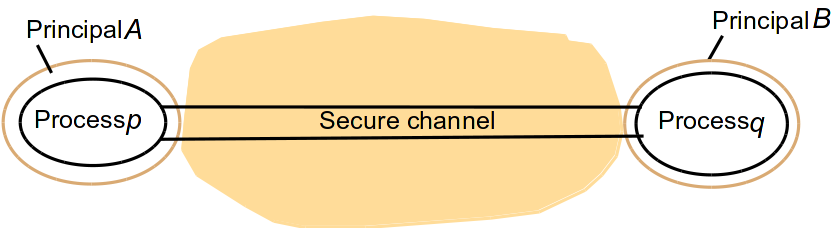
\includegraphics[scale=.4]{figs/seguranca4}
	\end{figure}
\end{frame}


% \frame[t]{
% 	\frametitle{Desafios Sistemas Distribuídos - Transparência}
% 
% 	A \alert{transparência} é a \textbf{ocultação da separação dos componentes} em um sistema distribuído de modo que o sistema seja percebido como \textbf{um todo}, em vez de \textbf{uma coleção de componentes independentes}. \textbf{Alguns tipos de transparências desejáveis em SD são:}
% 	\begin{itemize}
% 		 \item \alert{\textbf{Acesso}}: Entidades remotas e locais podem ser acessados usando operações idênticas.
% 		 \item \alert{\textbf{Localização}}: Entidades podem ser acessadas sem o conhecimento de sua localização.
% 		 \item \alert{\textbf{Migração}}: Entidades podem se deslocar sem afetar a operação dos usuários ou programadores.
% 		 \item \alert{\textbf{Replicação}}: Várias instâncias para aumentar a confiabilidade e desempenho.
% 		 \item \alert{\textbf{Falhas}}: Esconde dos programadores e usuários as falhas.
%      \end{itemize}
% }

\subsection{Transparência}

\begin{frame}
	\frametitle{Transparência}
	\begin{block}{}
	    \textbf{Esconder dos usuários} o fato que o\textbf{ processamento e os recursos estão fisicamente distribuídos} por diversos computadores
		\uncover<1->{
		\begin{itemize}
			\item O usuário deve enxergar como um único sistema
		\end{itemize}}
	\end{block}
	\begin{columns}[T]
		\column{.27\textwidth}
		\textbf{Tipo}
		\begin{itemize}
			\item \alert<3>{Acesso}
			\item \alert<4>{Localização}
			\item \alert<5>{Desempenho}
			\item \alert<6>{Mobilidade ou Migração}
			\item \alert<7>{Replicação}
			\item \alert<8>{Concorrência}
			\item \alert<9>{Falhas}
		\end{itemize}
		\column{.7\textwidth}
		\only<3>{\textbf{Entidades remotas e locais podem ser acessadas usando operações idênticas}
		\begin{itemize}
			\item Esconder as diferenças para representação dos dados
			\begin{itemize}
			    \item Como os dados serão representados em diferentes arquiteturas de máquinas e sistemas operacionais
			    \item Ex: Convenções para nomes de arquivos, bem como sua manipulação em diferentes sistemas operacionais
			    \begin{itemize}
				\item Usuários e aplicações não precisam ter ciência disto
			    \end{itemize}
			\end{itemize}
		\end{itemize}}
		\only<4>{\textbf{Esconder a localização dos recursos}
		\begin{itemize}
			\item Entidades podem ser acessadas sem o conhecimento de sua localização.
			\item Usuário não consegue determinar onde um recurso está localizado fisicamente no sistema
			\item Ex: \url{http://www.pb.utfpr.edu.br/favarim}
				\begin{itemize}
					\item Onde está localizado o servidor web da UTFPR?
				\end{itemize}
		\end{itemize}}
		\only<5>{\textbf{Permitir que o sistema seja reconfigurado para melhorar o desempenho de acordo com a carga}
		\begin{itemize}
			\item Novos servidores \textit{web} poderiam ser agregados para ajudar no balanceamento de carga em períodos críticos
			\item Ex: Último dia para entrega do IRPF
		\end{itemize}}
		\only<6>{\textbf{Esconder a mudança de localização enquanto os recursos estão sendo acessados}
		\begin{itemize}
			  \item Entidades podem se deslocar sem afetar a operação dos usuários ou programadores.
		\end{itemize}}
		\only<7>{\textbf{Esconder que os recursos são replicados}
		\begin{itemize}
			\item Recursos podem ser replicados para aumentar a disponibilidade ou desempenho
			\item Ex: Quando acessa a página do facebook ou google, em qual servidor você está se conectando? 
			\begin{itemize}
			 \item No mais próximo do teu computador ou no servidor no EUA? 
			\end{itemize}
		\end{itemize}}
		\only<8>{\textbf{Esconder que o recurso pode estar sendo compartilhado de forma concorrente com outros usuários}
 		\begin{itemize}
 			\item Dois usuários estão acessando simultaneamente a mesma tabela no Banco de Dados
% 			\item O sistema deverá garantir o acesso concorrente ao mesmo tempo que garante a consistência dos dados (geralmente protegidos por \textit{locks}) 
 		\end{itemize}}
		\only<9>{\textbf{Esconder as falhas de um recurso, bem como sua recuperação}
		\begin{itemize}
			\item Servidor web possui 3 réplicas para melhorar o desempenho
			\item Se uma réplica falhar, o serviço continua acessível
			\item Quando a réplica que falhou for recuperada, nada muda na forma de acesso para o usuário
		\end{itemize}}
	\end{columns}
\end{frame}



\begin{frame}[wide]
	\frametitle{Transparência}
	\begin{itemize}
		\item É \textbf{impossível} prover um sistema distribuído \textbf{completamente transparente}
		\begin{itemize}
			\item Impossível esconder a latência na transmissão pela Internet
			\item Nem sempre será possível esconder falhas do sistema
		\end{itemize}
		\item \textbf{Em alguns casos é desejável que o usuário tenha ciência}
		\begin{itemize}
			\item Ex: O usuário precisa saber onde está a impressora para onde mandou o trabalho
		\end{itemize}
	\end{itemize}
\end{frame}



\section{Arquiteturas de Sistemas Distribuídos}
\subsection{Definição}
\begin{frame}[t]
	\frametitle{Arquiteturas de Sistemas Distribuídos}
	\begin{block}{Arquitetura de Software}
		\begin{itemize}
			\item Originalmente, se referia à estruturação do software em camadas ou em módulos em um único computador;
			\item Atualmente, se refere à estruturação tanto no mesmo ou em computadores diferentes.
		\end{itemize}
	\end{block}

	\begin{block}{A arquitetura de um sistema distribuído:}
		\begin{itemize}
			\item é a sua estrutura em termos de componentes especificados separadamente 
			\item demonstra como os seus componentes interagem para chegar a um objetivo
			\item trata dos papéis funcionais e os padrões de comunicação
		\end{itemize}
	\end{block}
\end{frame}

\begin{frame}[t]
	\frametitle{Arquiteturas de Sistemas Distribuídos}
	\begin{block}{Plataforma}
		\begin{itemize}
		 	\item Termo utilizado para fazer referência a camadas de baixo nível de hardware e software que provêem serviços a camadas superiores;
			\item Normalmente, em termos de computadores, uma plataforma está relacionada ao tipo de arquitetura de processador e o sistema operacional utilizado.   
			\begin{itemize}
				\item Intel/Windows, Intel/Linux, PowerPC/MacOS, etc.
			\end{itemize}
		\end{itemize}
	\end{block}
	\begin{figure}
		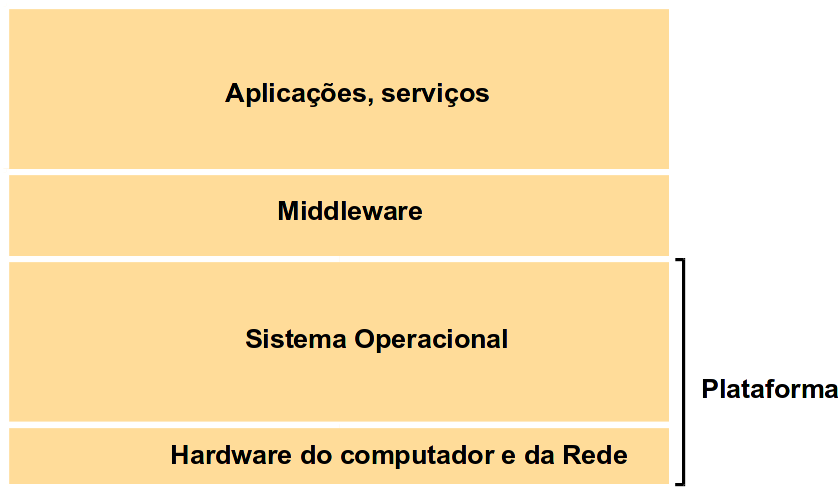
\includegraphics[scale=.2]{figs/middleware}
	\end{figure}
\end{frame}

\begin{frame}[t]
	\frametitle{Arquiteturas de Sistemas Distribuídos}
	\begin{block}{Middleware}
		\begin{itemize}
			\item termo aplicado para uma camada de software que tem o objetivo de providenciar uma abstração na programação através do ocultação das diferenças ({\color{blue}heterogeneidade}) existentes nos ambientes de rede, hardware, sistemas operacionais e linguagens de programação.
			\item oferece um modelo programação uniforme para os programadores, simplificando bastante o desenvolvimento de aplicações distribuídas;
			\item auxilia na obtenção das transparências desejáveis em SD;
			\item \alert{Exemplos:} RPC, RMI, CORBA, Serviços Web. 
		\end{itemize}
	\end{block}

	\begin{figure}
		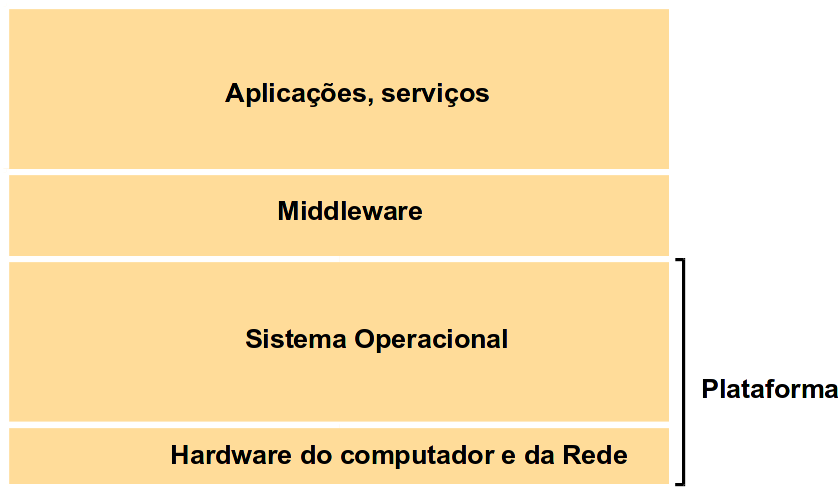
\includegraphics[scale=.2]{figs/middleware}
	\end{figure}
\end{frame}

\subsection{Papéis de Processos em Sistemas Distribuídos}
\begin{frame}[t]
	\frametitle{Arquiteturas de Sistemas Distribuídos}
	\begin{block}{Papéis de processos no SD:}
		\begin{itemize}
			\item \textbf{Processo servidor} - provê serviços, aceita pedidos de outros processos
			\item \textbf{Processo cliente} - utiliza serviços
			\item \textbf{Processo par} - Papel igualitário (prove e usa serviços)
		\end{itemize}
	\end{block}
\end{frame}


\section{Arquiteturas Típicas}
\frame[t]{\frametitle{Arquiteturas de Sistemas Distribuídos}
  \begin{block}{Arquiteturas Existentes:}
	    \begin{itemize}
	      \item \textbf{Cliente/Servidor e variações}
	      \begin{itemize}
		\item Mais usada em sistemas distribuídos
	      \end{itemize}
	      \item \textbf{Peer-to-Peer (P2P)}
	      \begin{itemize}
		\item Todos os envolvidos desempenham funções semelhantes, interagindo cooperativamente como pares (peers), sem distinção entre processos clientes e servidores.
	      \end{itemize}
	      \item \textbf{Híbrida:} Cliente/Servidor + P2P
	    \end{itemize}
	\end{block}
}

\subsection{Cliente/Servidor}
\frame[t]{\frametitle{Arquitetura Cliente/Servidor}
  \begin{itemize}
    \item Processos clientes invocam serviços aos servidores;
    \item Arquitetura mais comum e utilizada em SD.
  \end{itemize}
  \begin{figure}
    \centering
    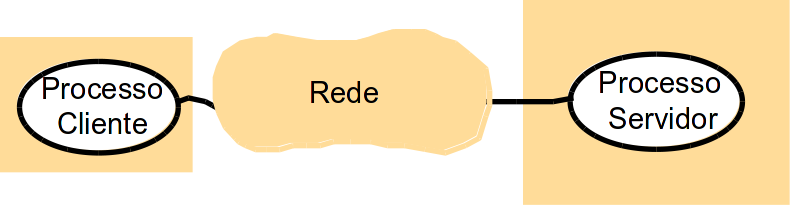
\includegraphics[scale=.4]{figs/cs1}
  \end{figure}
}

\frame[t]{\frametitle{Variação: Arquitetura Cliente/Servidor}
  \begin{block}{Servidor como cliente de outro servidor}
    Neste modelo, um servidor pode se tornar um cliente para solicitar serviços de outro servidor. Ex:
  \begin{itemize}
    \item Um servidor de email busca no DNS o endereço IP de outro servidor de email;
    \item Um serviço de busca on-line de passagens em várias companias aéreas.
  \end{itemize}
  \end{block}  \begin{figure}
    \centering
    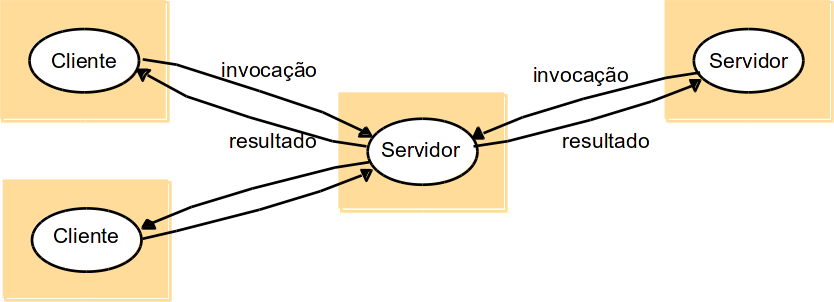
\includegraphics[scale=.4]{figs/cs2}
  \end{figure}
}

\frame[t]{\frametitle{Variação: Arquitetura Cliente/Servidor}
  \begin{block}{Serviço fornecido por múltiplos servidores}
    Neste modelo, os serviços são implementados em vários servidores (réplicas) que interagem entre si para oferecerem os serviços solicitados pelos processos clientes.
  \end{block}
  \begin{figure}
    \centering
    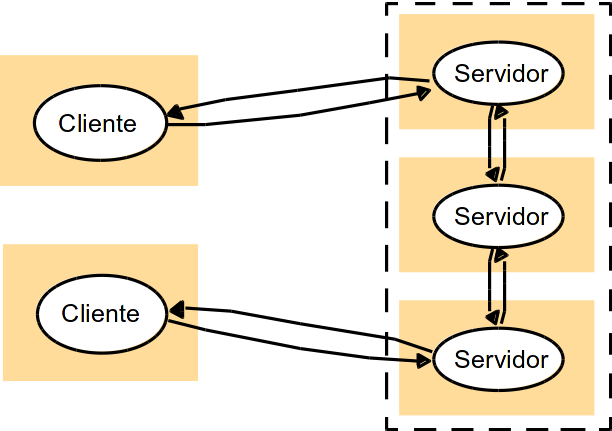
\includegraphics[scale=.35]{figs/cs3}
  \end{figure}
}

\frame[t]{\frametitle{Variação: Arquitetura Cliente/Servidor}
  \begin{block}{Servidor Proxy}
    \begin{itemize}
     \item Servidores proxy mantêm cópias de dados solicitados anteriormente. 
     \item Quando um cliente faz uma solicitação a um servidor proxy, primeiro é verificado se os dados estão presentes localmente, caso contrário a informação é buscada efetivamente na rede.
     \item O propósito geral é garantir desempenho e disponibilidade de dados sem aumentar a carga ou tráfego na rede utilizada.
    \end{itemize}
  \end{block}  
  \begin{figure}
    \flushleft
    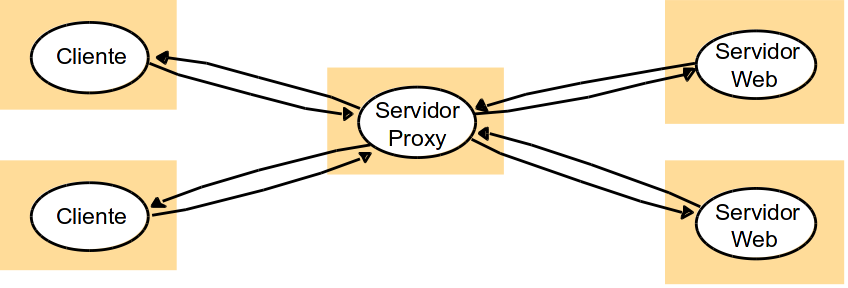
\includegraphics[scale=.33]{figs/cs4}
  \end{figure}
}

\frame[t]{\frametitle{Variação: Arquitetura Cliente/Servidor}
  \begin{block}{Código Móvel}
    Seu funcionamento é baseado de modo a permitir que os códigos sejam transferidos do servidor para o cliente, onde são executados. (\alert{vantagem: sem atraso/sem tráfego}). Ex:applets
  \end{block}
  a) cliente requisita o download do código do applet
  \begin{figure}
    \centering
    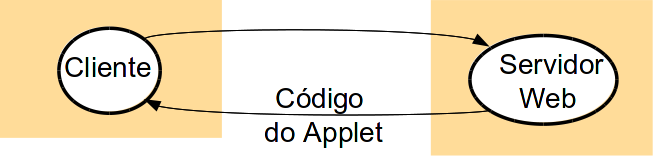
\includegraphics[scale=.35]{figs/cs5-applet}
  \end{figure}
b) cliente interage com o applet
  \begin{figure}
    \centering
    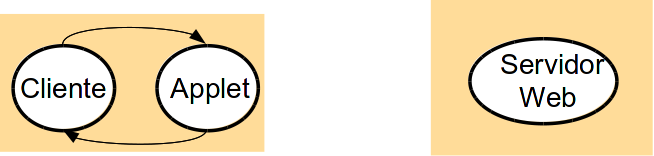
\includegraphics[scale=.35]{figs/cs6-applet}
  \end{figure}
}


\frame[t]{\frametitle{Variação: Arquitetura Cliente/Servidor}
  \begin{block}{Código Móvel}
    Através de códigos móveis é possível oferecer serviços que não podem ser dado normalmente pela Web (modelo \textbf{pull} de comunicação). Ex:
    \begin{itemize}
      \item Serviços de mensagens do tipo \textbf{push}
      \item O servidor inicia a comunicação
    \end{itemize}
  \end{block}
}

\frame[t]{\frametitle{Variação: Arquitetura Cliente/Servidor}
  \begin{block}{Agentes Móveis}
    São programas executáveis (\textbf{códigos e dados}) que trafegam de um computador ao outro para executar alguma tarefa. \alert{Ex:} Aplicações que necessitem coletar diversas informações em muitas máquinas.
    \begin{itemize}
     \item A vantagem é a redução do tráfego de rede, devido a redução de número de chamadas remotas por parte de códigos fixos;
    \end{itemize}
  \end{block}
  \begin{figure}
    \centering
    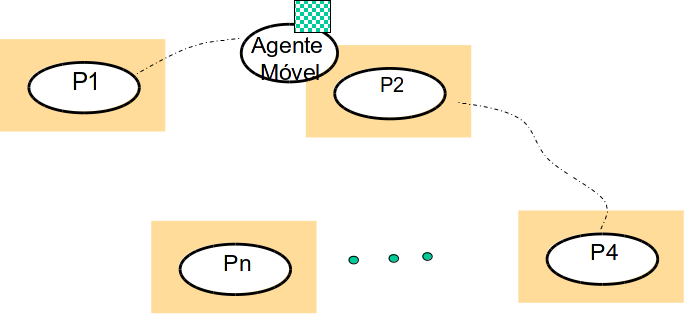
\includegraphics[scale=.38]{figs/cs7-agente}
  \end{figure}
}

\frame[t]{\frametitle{Variação: Arquitetura Cliente/Servidor}
  \begin{block}{Agentes Móveis}
    Cuidados com a segurança:
    \begin{itemize}
      \item O ambiente deve preocupar como e quais recursos pode prover aos agentes móveis. 
      \item Por outro lado, os agentes também podem sofrer problemas e não completarem suas tarefas, pois não conseguiram ter acesso autorizado aos recursos necessários.
    \end{itemize}
  \end{block}
}

\frame[t]{\frametitle{Variação: Arquitetura Cliente/Servidor}
  \begin{block}{Thin Clients}
      O termo ``\textit{thin client}'' consiste da arquitetura em que os aplicativos são executados em um computador \alert{remoto (servidor)}.
    \begin{itemize}
      \item Diferente da arquitetura de computadores de rede, os aplicativos são todos executados nos servidores e não baixados;
      \item Servidores devem ser poderosos, capazes de executar diversos processos em paralelo para atender inúmeros clientes.
    \end{itemize}
  \end{block}
  \begin{figure}
    \flushleft
    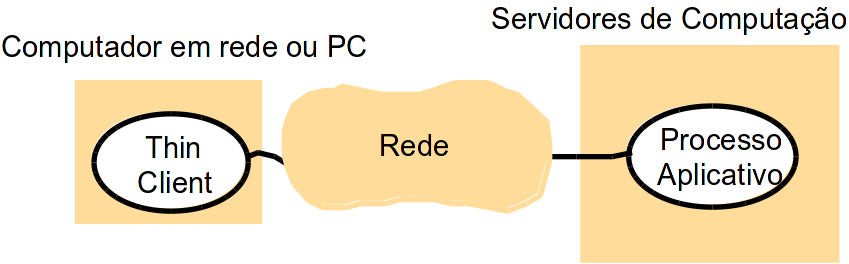
\includegraphics[scale=.35]{figs/cs8-thinclient}
  \end{figure}

}

\subsection{Peer-to-Peer}
\frame[t]{\frametitle{Arquitetura Peer-to-Peer}
  \begin{block}{}
    \begin{itemize}
      \item Nesta arquitetura todos processos interagem com regras \textbf{semelhantes}; 
      \item Trabalham de forma \textbf{cooperativa} para desempenhar atividades computacionais; 
      \item \alert{Não há distinção entre cliente e servidor} - papel igualitário.
      \item Exemplo: GnuTella
    \end{itemize}


  \end{block}
  \begin{figure}
    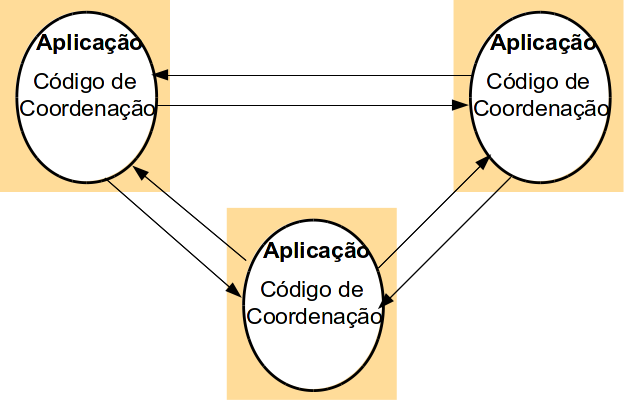
\includegraphics[scale=.34]{figs/p2p}
  \end{figure}
}

\subsection{Híbrida}
\frame[t]{\frametitle{Arquitetura Hibrida}
  \begin{block}{}
    Combina aspectos da arquitetura cliente/servidor e peer-to-peer. \alert{Ex:}
    \begin{itemize}
     \item Mensagem instântanea
     \item Algumas arquiteturas de compartilhamento de arquivos: napster, bittorrent. 
    \end{itemize}

  \end{block}
  \begin{figure}
    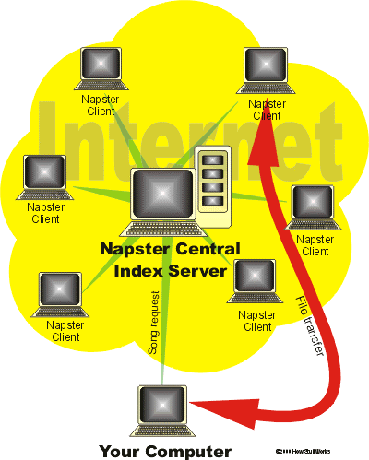
\includegraphics[scale=.34]{figs/napster}
  \end{figure}
}


\frame[t]{ \frametitle{Próxima aula}
	 \begin{itemize}
	  \item Revisão: Programação de aplicações locais orientadas a objetos em java
	 \end{itemize}
}

\end{document}
